\section{Tweedimensionale stapelproblemen}

\subsection{Algemeen}
In de voorbije lessen hebben we het vooral gehad over complete vlakvullingen, i.h.b. het vullen van vlakken met vierkanten. 
In dit onderdeel zullen we kijken naar het vullen van vlakken met figuren die het vlak nooit volledig zullen vullen. We noemen dit dan een tweedimensionale stapelprobleem. We zijn namelijk op weg om het bolstapelprobleem van Kepler te bekijken!

Bij het stapelen in twee dimensies hebben we minder mogelijkheden dan bij het stapelen in drie dimensies, maar we kunnen er toch heel veel over zeggen. Als we denken aan tweedimensionale stapelingen, dan denken we aan een vlak waarin we voorwerpen stapelen die twee dimensies hebben. Deze voorwerpen kunnen heel uiteenlopend zijn. Naar analogon met het bolstapelprobleem van Kepler waarbij we met bollen zullen werken bekijken we het geval van de cirkels. 


In de eerste les hebben we reeds gezien dat je een oneindig vlak volledig kan vullen met identieke gelijkzijdige driehoeken, vierkanten en zeshoeken. Dit noemen we 100\% effici�ntie. 

\ask{Hebben we ook 100\% effici�ntie als we een oneindig vlak zouden betegelen met cirkels?}

\answer[2cm]{Neen, want cirkels hebben geen rechte zijde om ze aan elkaar te plaatsen.}

Het antwoord is natuurlijk 'neen'. Maar wat is de effici�ntie dan wel? En in welke configuratie is deze het beste?

\task{Probeer cirkels (munten, flippo's, pokerjetons ...) eens zodanig op een tafel te leggen dat er zo weinig mogelijk ruimte tussen de cirkels overblijft.}

Het was reeds duidelijk je nooit elk plekje van de tafel kunt bedekken als de cirkels elkaar niet mogen overlappen.

We zijn in eerste instantie ge�nteresseerd in rangschikkingen van oneindig veel cirkels op een oneindige grote tafel. Je hoeft dan geen rekening te houden met wat er aan de randen gebeurt. De randen maken alles moeilijker (maar ook interessanter, iets waar we later nog op zullen terug komen). E�n voor de hand liggende mogelijkheid om de cirkels zo effici�nt mogelijk in het vlak te rangschikken is om ze netjes naast en boven elkaar te leggen, volgens een patroon van vierkantjes. Dat dit niet de best mogelijke oplossing is wordt al snel duidelijk door wat met de rijen te schuiven. Je kunt de rijen namelijk iets beter in elkaar laten passen. Iedere cirkel raakt dan aan zes andere cirkels \todo{Vermelden van kissingnumber?}, in plaats van aan vier, zoals in het vierkante geval. De cirkels komen nu in een regelmatig patroon te liggen op een zogenaamd hexagonaal rooster. Het lijkt onmogelijk om de cirkels nog dichter bij elkaar te krijgen. Dat dit inderdaad niet beter kan werd ongeveer honderd jaar geleden bewezen door de Deense getaltheoreticus Thue. Een schets van het bewijs zullen we zo meteen bekijken. Eerst gaan wij zelf op zoek naar wat nu juist de effici�ntie is en hoe je deze moet berekenen.

\subsection{Voronoicellen}

Om te berekenen hoe effici�nt een schikking met cirkels is, maken we gebruik van Voronoicellen. De {\bf Voronoicel} van een cirkel is de verzameling van alle punten die dichter bij het middelpunt van deze cirkel liggen dan bij het middelpunt van elke andere cirkel in de schikking.

\ask{Hoe ziet de Voronoicel eruit bij een vierkante rangschikking? Hoe ziet de Voronoicel eruit bij de hexagonale rangschikking?}

\answer[2cm]{Bij de vierkante rangschikking is zo'n Voronoicel een vierkant dat strak om de cirkel zit, en voor de hexagonale rangschikking is het een regelmatige zeshoek.}

\ask{Hoe kan je de effici�ntie berekenen aan de hand van zo'n Voronoicel?}

\answer[3cm]{Het percentage van het vlak dat wordt bedekt door de cirkels is gelijk aan het percentage van de Voronoicel dat door ��n cirkel wordt bedekt, want voor alle cirkels is de vorm van de Voronoicel hetzelfde en de Voronoicellen betegelen samen het hele vlak.}

\task{Bereken voor de vierkante en de hexagonale rangschikking de effici�ntie.}

\begin{enumerate}
	\item \textbf{Vierkante rangschikking}:\\
	\answer[2cm]{Als je cirkels neemt met straal gelijk aan 1, dan heeft het strakke 'omgeschreven' vierkant in de vierkante betegeling een zijde met lengte 2. De oppervlakte van de cirkel hier is $\pi$, de oppervlakte van het vierkant is 4. (Uiteraard konden we andere afmetingen genomen hebben, maar de verhoudingen blijven steeds hetzelfde.) Er is dus $\frac{\pi}{4}=0,78538...$, of ruim 78\% van het totale vlak bedekt door de cirkels.}
	\item \textbf{Hexagonale rangschikking}:\\
	\answer[2cm]{De zeshoek om een cirkel met straal 1 kan worden opgedeeld in twaalf halve gelijkzijdige driehoekjes met een basis met lengte 1 en een hoogte van $\frac{1}{\sqrt{3}}$. De oppervlakte van de zeshoek is dus $12.\frac{1}{2}.1.\frac{1}{\sqrt{3}}=2\sqrt{3}$. De effici�ntie of bedekkingsgraad is dus $\frac{\pi}{\sqrt{12}}=0.90689$.}
\end{enumerate}


\begin{figure}[h]
  \centering
  \subfloat[]{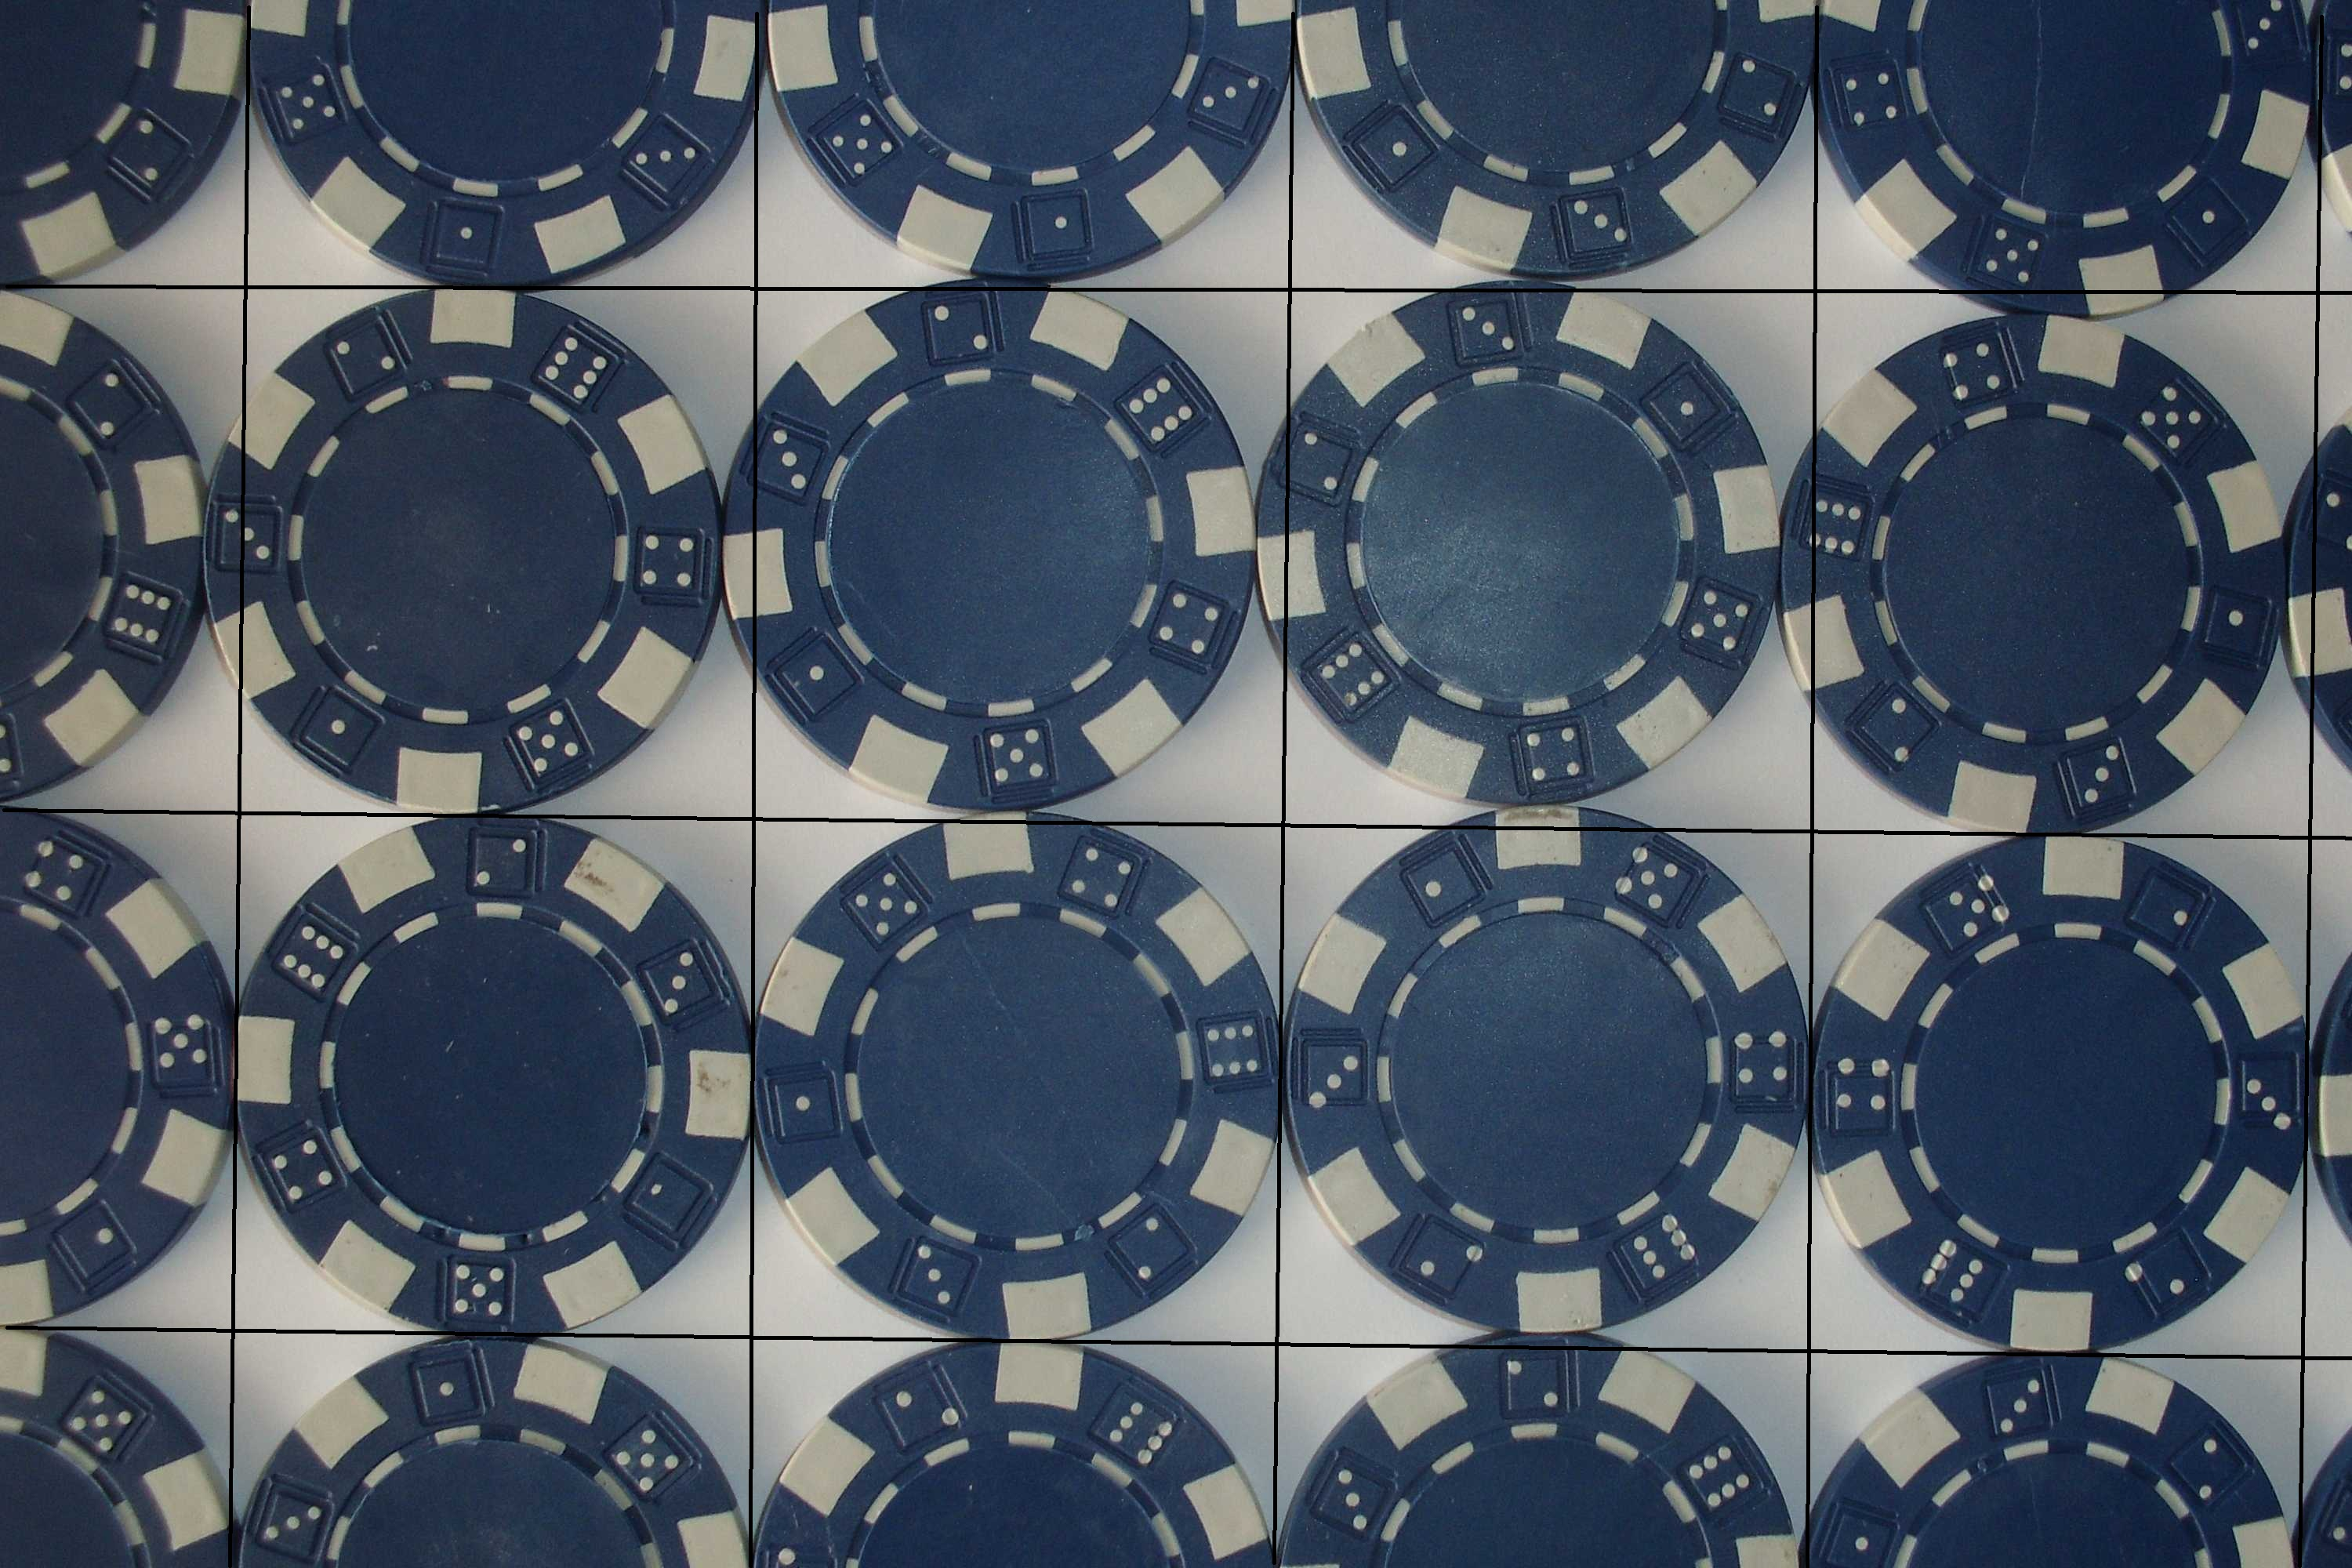
\includegraphics[width=0.45\textwidth]{voronoi_sqr}\label{vs}}\qquad
  \subfloat[]{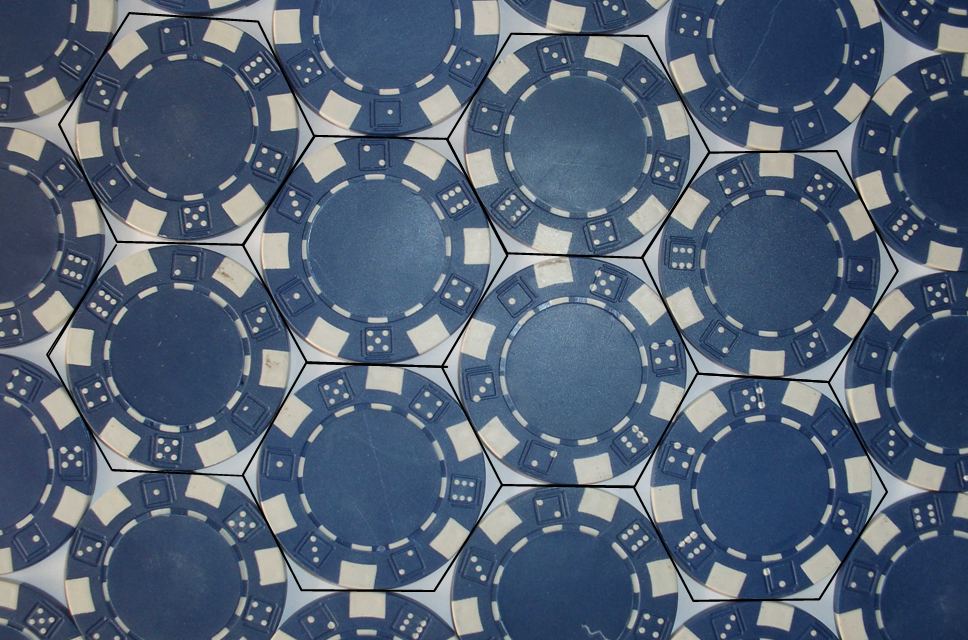
\includegraphics[width=0.45\textwidth]{voronoi_hex}\label{vh}}
  \caption{Vierkante en hexagonale rangschikking met pokerjetons en hun voronoicellen}  
\end{figure}


\subsection{Axel Thue}
De Scandinavische wiskundige Axel Thue (1863-1922) ontwikkelde in 1892 een theorie over het tweedimensionale equivalent voor 'het probleem van Kepler' waarin men zocht naar de dichtste pakkingsmethode voor cirkels in het vlak. Thue betegelde het vlak met identieke gelijkzijdige zeshoeken en tekende in elke zeshoek een cirkel op zo'n manier dat elke cirkel alle zijden van de zeshoek raakte. Hierdoor verkreeg hij een dichtheid van 90.69\%, waarvan hij beweerde dat dit de hoogst mogelijke dichtheid was bij het stapelen in 2 dimensies. 
Om dit te bewijzen tekende Thue een begrensd aantal cirkels met straal 1 die elkaar niet overlapten. Daarna verdeelde hij willekeurig het tweedimensionale vlak in bepaalde gebieden waarbij hij aantoonde dat de dichtheid in elk gebied maximum 90.69\% is. Hierdoor bestond er geen tweedimensionale pakking waarbij de dichtheid groter is dan 90.69\% en op die manier bewees Thue zijn vermoeden dat de hexagonale pakking de dichtste pakkingsmethode was in twee dimensies.
Het volledige bewijs zullen we hier niet meer bespreken, maar we zullen wel even kijken hoe Thue het vlak waarin de cirkels liggen heeft opgedeeld in verschillende gebieden. Hiervoor zullen we een korte vertaling geven van een deel van het oorspronkelijke Engelstalige bewijs dat geschreven is door Axel Thue.

\begin{quotation}
``Teken een grotere cirkel met straal $\frac{2}{\sqrt{3}}$ rond elke cirkel (zie figuur \ref{2D1}). Telkens als twee van deze grote cirkels elkaar snijden, teken je het lijnstuk tussen de twee snijpunten, waarna je twee congruente driehoeken construeert met het lijnstuk als basis en de tophoeken in het centrum van de cirkels (zie figuur \ref{2D2}). Er zal nooit een punt zijn dat tegelijk binnen alle drie de cirkels ligt. Zoals we merken in figuur \ref{2D3} zullen drie grote cirkels elkaar maximum in ��n punt snijden, het cirkelcentrum, als de centra van de drie grote cirkels de tophoeken zijn van een gelijkzijdige driehoek met zijde 2. \\
Dit geeft ons de verdeling van de ruimte: gebieden buiten de grote cirkels (wit), de gelijkbenige driehoeken (groenachtig blauw), en het gedeelte binnen de grote cirkels, maar buiten de driehoeken (lichtpaars) (zie figuur \ref{2D4}).''
\end{quotation}


\begin{figure}[h]
  \centering
  \subfloat[]{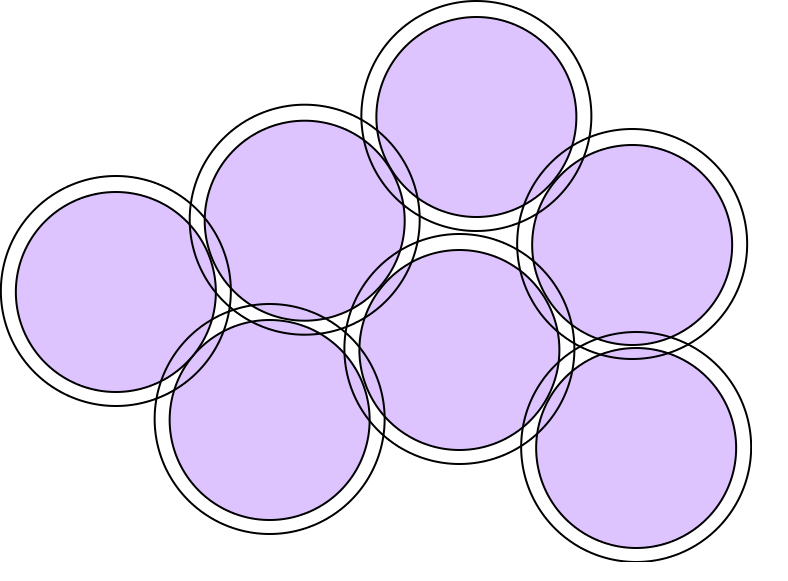
\includegraphics[height=3cm]{2D1}\label{2D1}}
  \subfloat[]{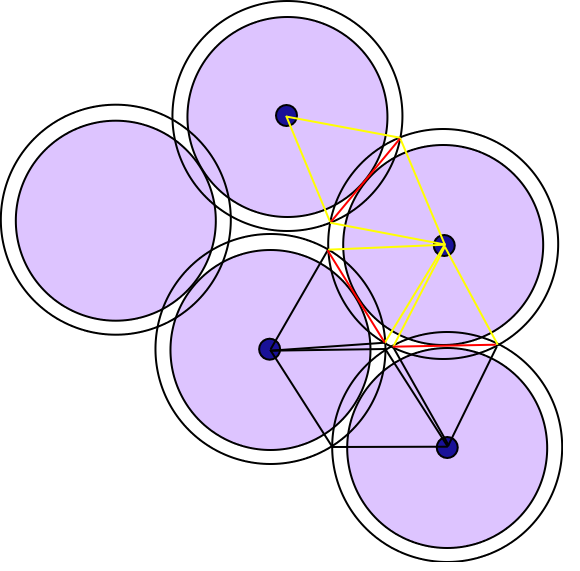
\includegraphics[height=3cm]{2D2}\label{2D2}}
  \subfloat[]{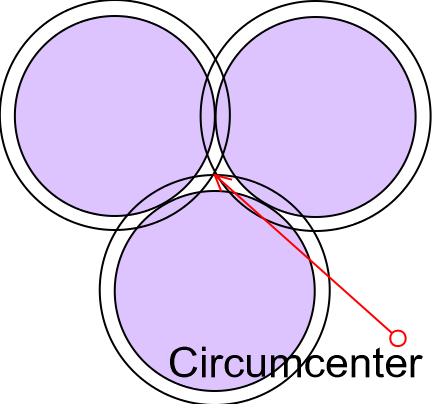
\includegraphics[height=3cm]{2D3}\label{2D3}}
  \subfloat[]{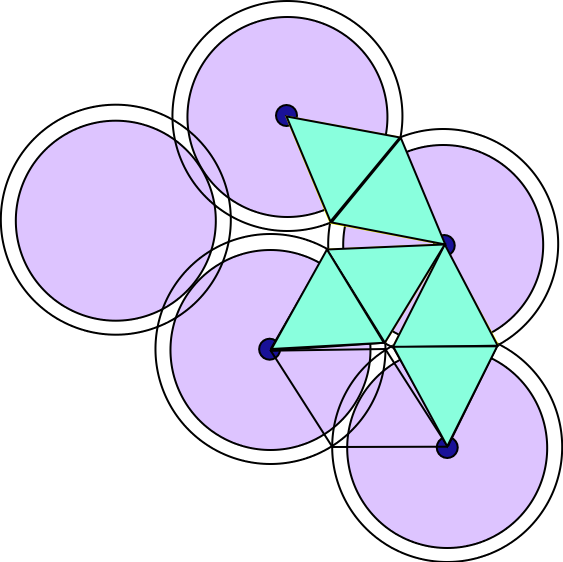
\includegraphics[height=3cm]{2D4}\label{2D4}}\\
  \caption{Figuren bij bewijs van Axel Thue}  
\end{figure}

Uit deze vertaling concluderen we dus dat Thue zijn vlak in 3 gebieden opgedeeld heeft. Hierna zal hij nog berekenen hoeveel oppervlakte er in de drie gebieden wordt ingenomen door de cirkels en uiteindelijk zal hij tot de conclusie komen dat geen enkel gebied een dichtheid heeft van meer dan 90.69\%, waardoor het bewijs voor het tweedimensionale equivalent van het bolstapelprobleem is afgerond.


\subsection{Dienbladenprobleem}
Bij de meeste stapelingen stelt men zich de vraag hoeveel identieke voorwerpen men in een ruimte met vastgelegde grenzen kan stoppen. Wij zullen de vraag omkeren. In ons praktische probleem vragen we ons af wat de meest compacte ruimte is voor een vastgelegd aantal identieke voorwerpen.
We kunnen dit probleem als volgt bekijken: een fabrikant wil dienbladen voor een bepaalde aantal glazen of blikjes. Hij wil dus weten hoe groot zo'n dienblad moet zijn zodat er precies 1,2,3 ... glazen of blikjes op passen. Omdat de fabrikant ruimdenkend is, wil hij niet enkel de traditionele cirkelvormige dienbladen uitproberen, maar ook rechthoekige of zeshoekige dienbladen. 

\task{Bepaal nu voor welke hoeveelheid glazen of blikjes we welk soort dienblad willen maken en wat juist de effici�ntie is, m.a.w. hoeveel procent van het dienblad dat gevuld zal zijn. Schrijf dit in onderstaande tabel.}


\begin{table}[h]
\centering
\begin{tabular}{l||c|c|c|c}
Aantal / vorm & cirkelvormig & driehoekig & rechthoekig& zeshoekig\\\hline\hline
1&&&&\\\hline
2&&&&\\\hline
3&&&&\\\hline
4&&&&\\\hline
5&&&&\\\hline
6&&&&\\\hline
7&&&&\\\hline
8&&&&\\\hline
9&&&&\\\hline
10&&&&\\\hline
11&&&&\\\hline
12&&&&\\\hline
13&&&&\\\hline
...&&&&\\
\end{tabular}
\caption{De effici�ntie van de dienbladen bij een bepaalde hoeveelheid glazen of blikjes}
\label{}
\end{table}

Het is nu de bedoeling dat jullie deze tabel gaan proberen in vullen door zelf te gaan experimenteren. Het probleem van de glazen kunnen we gaan voorstellen met munten en de dienbladen gewoon als een veelhoek.

\task{Gebruik het bijgeleverde Geogebra-applet om experimenteel de effici�ntie te bepalen.}

\teacher{Eerst en vooral hebben we de geogebra-applet. Hier kunnen de leerlingen zelf met fictieve munten en verstelbare dienbladen gaan uitproberen, waarbij de effici�ntie gewoon voor hen wordt uitgerekend. Het is wel  nodig dat de leerlingen telkens aanduiden voor welke hoeveelheid munten ze de effici�ntie aan het bepalen zijn. Dit is vooral de bedoeling voor het cirkelvormig en zeshoekig dienblad. Ook kan dit gedaan worden voor het rechthoekig en/of driehoekig dienblad.}

\task{Neem een rechthoekig stuk karton en knip hierug een gelijkzijdige driehoek weg. Plaats dan munten of pokerjetons in het lege gebied. Schuif nu de jetons met een liniaal in de richting van het bovenste hoekpunt. Houd de liniaal z� dat de munten telkens in een gelijkzijdige driehoek zitten. De munten zitten zo in een gelijkzijdige driehoek die je zo klein mogelijk probeert te maken. Soms moet je de munten met je vingers een beetje helpen om ze op een goede plek te krijgen. Probeer de munten in een zo klein mogelijke driehoek te krijgen. Nu bereken je de effici�ntie van je opstelling.}

\teacher{Om de effici�ntie te berekenen zullen de leerlingen de oppervlakte van de gelijkbenige driehoek die wordt bekomen met de liniaal moeten delen met de oppervlakte van alle jetons.}

\todo{Pieter, zou jij zo een karton willen maken en daar dan gewoon enkele pokerjetons in willen leggen en een foto van trekken (de pokerjetons nog niet in de optimale configuratie leggen, maar gewoon willekeurig)?}.

\task{Ook voor het rechthoekig dienblad gebruik je een stuk karton. Als je twee keer een rechte hoek uitknipt, dan kan je hiermee een rechthoek maken. Ook gebruikmaken van 4 linialen (en een geodriehoek) kan lukken. Leg dan binnen dit rechthoekig dienblad een aantal jetons en bereken de effici�ntie die je bekomt.}

\teacher{Bij deze opdracht is het ook de bedoeling dat de leerlingen effectief de effici�ntie in sommige gevallen exact gaan uitrekenen door berekeningen. Het is aan de leerkracht om op voorhand te zeggen dat de leerlingen ofwel voor bijvoorbeeld 3 gevallen dit moeten uitrekenen, ofwel bijvoorbeeld voor de specifieke gevallen 'een driehoekig dienblad met 3 munten' en 'een zeshoekig dienblad met 7 munten'.}

Het is ook de bedoeling dat jullie voor enkele gevallen de effici�ntie ook exact gaan uitwerken d.m.v. berekeningen en een goede figuur.

Vooraf is het dan misschien handig om eerst enkele formules op te frissen:

\begin{itemize}
  \item Oppervlakte cirkel met straal $r$: $\pi.r^2$
	\item Oppervlakte driehoek met basis $b$ en hoogte $h$: $\frac{b.h}{2}$
	\item Oppervlakte rechthoek met lengte $l$ en breedte $b$: $l.b.$
	\item Oppervlakte regelmatige $n$-hoek met zijde $z$: $\frac{1}{2}.n.z^2.\sin(\frac{2\pi}{n})$
	\item Oppervlakte regelmatige zeshoek met zijde $z$: $\frac{3}{2}.z^2.\sqrt{3}$
	\item \ask{Hoogte in gelijkzijdige driehoek met zijde $b$:} \answer{$\sqrt{b^2-(\frac{b^2}{2})^2}$}	
\end{itemize}

\teacher{Indien de formule voor de regelmatige zeshoek niet gekend is, is het goed dit samen eerst met de leerlingen te bepalen.}

In de volgende sectie zullen wij enkele gevallen effectief uitrekenen.

\todo{PP: hier ben ik gekomen met lezen, to be continued..}

\subsubsection{Berekeningen voor enkele specifiek gevallen}

Wij zullen voor de berekeningen gebruik maken van de afmetingen van een jeton met een straal van 2 cm. Deze afmetingen zijn ook zo bij de geogebra-applets \todo{Dit aanpassen}.
De oppervlakte van 1 jeton is $4*\pi\approx 12,5664$. Omdat we voornamelijk ge�nteresseerd zijn in de optimale compactheid van een dienblad en waarbij hier een resultaat van ... \todo{voorbeeld zoeken van absurd resultaat} geen betekenis heeft, zullen we steeds de afmetingen afronden op 4 cijfers na de komma en de percentage tot op de honderdtallen.
We zullen dus bij elk voorbeeld duidelijk de oppervlakte van de jetons, de oppervlakte van het dienblad en de effici�ntie. Dit laatste is de hoeveel van de oppervlakte van het dienblad die de munten innemen, uitgedrukt in percentage, en deze wordt berekend door de oppervlakte van de munten te delen door de oppervlakte van het dienblad en dit te vermenigvuldigen met 100.


\begin{vb}[Dienbladen met 1 munt]

\begin{figure}[h]
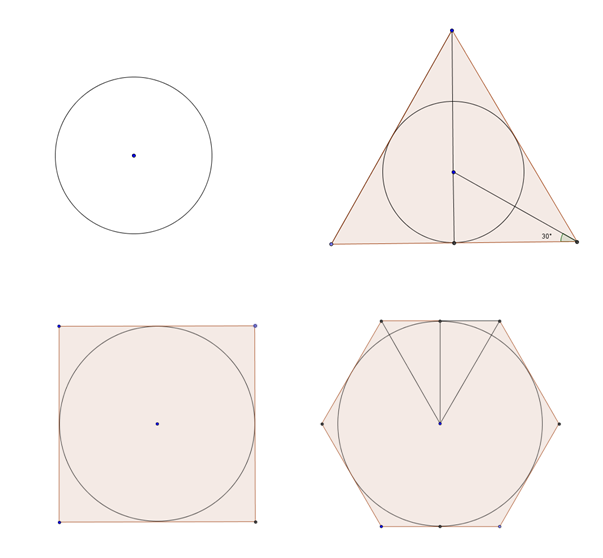
\includegraphics[width=10cm]{1munten}
\caption{De dienbladen voor 1 munt}
\label{1munt}
\end{figure}

\begin{itemize}
	\item \textbf{Cirkelvormig dienblad:} \\
	Wanneer we slechts 1 munt hebben, is een cirkelvormig dienblad het effici�nst, omdat er dan geen vrije ruimte meer overblijft. E�n munt neemt dus 100\% van de oppervlakte van het cirkelvormig dienblad in. We kunnen dit als volgt samenvatten:
	
	\begin{itemize}
	\item Oppervlakte dienblad = 12,5664 cm$^2$
	\item Effici�ntie = 100\%
\end{itemize}
	
	\item \textbf{Driehoekig dienblad:}\\
	Bij een driehoekig dienblad is de lengte van de basis gelijk aan $2.2.\tan(\pi/6)=4\sqrt{3}\approx 6,9282$. De hoogte is $\sqrt{b^2-(\frac{b}{2})^2}= 6$. Daaruit volgt dat:
	\begin{itemize}
	\item Oppervlakte dienblad = $20,7846$ cm$^2$
	\item Effici�ntie = 60,46 \%
\end{itemize}	

	\item \textbf{Rechthoekig dienblad:}\\
	De oppervlakte van de meest compacte rechthoek voor 1 jeton is niet moeilijk te vinden. Aangezien we zien dat de lengte en de breedte beide gelijk zijn aan de diamter van de munt, weten we dat:
	
	\begin{itemize}
	\item Oppervlakte dienblad = $16$ cm$^2$
	\item Effici�ntie = 78,54\%
\end{itemize}
	
	\item \textbf{Zeshoekig dienblad:}\\
	Voor de oppervlakte van de gelijkzijdige zeshoek te berekenen, moeten we de straal van deze zeshoek berekenen (of zijde, die daaraan gelijk is). Deze is gelijk aan de straal van de jeton gedeeld door $\cos(\pi/6)$. Dus in de formule $\frac{3}{2}.z^2.\sqrt{3}$ is $z=2,3094$ en vinden we dus dat de oppervlakte van de zeshoek gelijk is aan 13,8564 cm$^2$. 
	
	\begin{itemize}
	\item Oppervlakte dienblad = 13,8564 cm$^2$
	\item Effici�ntie = 90,69\%
\end{itemize}
\end{itemize}

\end{vb}

\begin{vb}[Dienbladen met 2 munten]
De oppervlakte van 2 munten is dus steeds $8.\pi\approx 25,1327$.
We zullen ook vanaf nu de berekeningen iets compacter schrijven.

\begin{itemize}
  \item \textbf{Cirkelvormig dienblad:}\\
  Om de oppervlakte te berekenen hebben we de straal van de grote cirkel nodig. Die is twee maal de straal van de munten en dit is $4$.  Hieruit volgt
  \begin{itemize}
	  \item Oppervlakte dienblad = $16\pi\approx 50,2655$ cm$^2$
	  \item Effici�ntie = 50\%
  \end{itemize}
  
	\item \textbf{Driehoekig dienblad:}\\
	De configuratie op de figuur geeft dezelfde als de configuratie met een munt in de rakende in de tophoek (je kan dit inzien door de figuur te draaien).
	De grootte van basis van de driehoek is gelijk aan twee keer de grootte van de projectie van het lijnstuk $[AB]$ (op de figuur), dus twee keer de grootte van $[AC]$, en de lengte van $[BD]$. Deze laatste is twee keer de straal van de jetons, dus gelijk aan 4, omdat de cirkels elkaar juist raken. De grootte van $[AC]$ heeft grootte $2\sqrt{3}$ zoals bij de berekeningen van het voorbeeld met 1 munt. De grootte van de basis is dus gelijk aan 4+4$\sqrt{3}\approx 10,9282$. Met deze basis weten we dat de hoogte van de driehoek 9,4641 is. Hieruit vinden we :
	
	\begin{itemize}
	\item Oppervlakte dienblad = 51,7128 cm$^2$.
	\item oppervlakte dienblad = 48,60\%
\end{itemize}
	
	
	\item \textbf{Rechthoekig dienblad:}\\
	De rechthoek die de 2 munten omvat heeft een lengte van 4 keer de straal van de munten en de breedte is gewoon de diameter. Zo vinden we dus :
	\begin{itemize}
	\item Oppervlakte dienblad = 32
	\item Compactheid dienblad = 78,54\%
\end{itemize}
	
	\item \textbf{Zeshoekig dienblad:}\\
	\todo{pfff, dat is hier een moeilijk ...}
	Om de straal van ons zeshoekig dienblad te berekenen hebben we een 'kleine' omweg genomen. In de driehoek $GIJ$ geldt dat de lengte van de zijde $JI$ gelijk is aan $\sqrt{R^2+R^2-2.R.R.\cos(150�)}=3,3859$ cm, waarbij we gebruik maken van de cosinusregel met $R$ de straal van de munten. Het lijnstuk $LI$ is even groot, waaruit volgt dat de driehoek $IJL$ gelijkbenig is. Hierbij weten we ook dat de hoek $L\hat{I}J$ $30�$ is, waardoor de hoek $I\hat{L}J$ $75�$ is. Hieruit volgt dat de hoek $A\hat{L}I$ 
	\begin{itemize}
	\item Oppervlakte dienblad = 
	\item Compactheid dienblad =
\end{itemize}
\end{itemize}

\todo{figuur}
\end{vb}


\begin{vb}[Dienblad met 3 munten]
De oppervlakte van 3 munten is gelijk aan $12\pi\approx 37,70$ cm$^2$.

\begin{itemize}
  \item \textbf{Cirkelvormig dienblad:}\\
  De straal van de cirkel is deze keer gelijk aan de som van de lengtes van twee lijnstukken, HA en AD. De lengte van HA is gelijk aan de straal van de munten. De lengte van AD vinden we in de driehoek ABC. Doordat deze driehoek gelijkzijdig is, geldt dat de hoogtelijnen elkaar in 1 punt snijden, het hoogtepunt. En dit punt verdeelt elke hoogtelijn van de driehoek in twee delen waarvan het ene deel twee keer zo groot is als het ander. Met andere woorden, de lengte van AD is twee keer de lengte van DE. Doordat de lengte van AE=$\sqrt{|AB|^2-|BE|^2}=\sqrt{16-4}=\sqrt{12}\approx 3,4641$ cm, is de lengte van AD gelijk aan 2,31cm. Hieruit volgt dat de straal van het cirkelvormig dienblad een lengte van 4,31 cm heeft, waaruit volgt dat :
  
  \begin{itemize}
	\item Oppervlakte dienblad = 58,36 cm$^2$.
	\item Compactheid dienblad = 64,62 \%
\end{itemize}
     
	\item \textbf{Driehoekig dienblad:}\\
	Aangezien het driehoekige dienblad bij drie munten hetzelfde is als dat bij twee munten hoeven we de berekeningen niet opnieuw te doen. We weten dus dat:
	
	\begin{itemize}
	\item Oppervlakte dienblad = 14,80 cm$^2$.
	\item Compactheid dienblad = 72,90 \%
\end{itemize}
	
	\item \textbf{Rechthoekig dienblad:}\\
	\item \textbf{Zeshoekig dienblad:}\\
	Om de straal van de zeshoek ABCDEF te verkrijgen berekenen we eerst de lengte van het rode lijnstuk. Dit rode lijnstuk is in twee gelijke delen verdeeld (FH en HB). Deze delen hebben een lengte die gelijk is aan de hoogte van de meest compacte gelijkzijdige driehoek bij 1 munt min 1 keer de straal van de munt (Dit kan je zien door bijvoorbeeld de driehoek die vertrekt in top B te beschouwen met de meest linkse cirkel). Dus $|HB|=|FH|=$
	
\end{itemize}
\end{vb}

\begin{vb}

\begin{itemize}
  \item \textbf{Cirkelvormig dienblad:}\\
  Om de oppervlakte te berekenen 
   \begin{itemize}
	\item Oppervlakte dienblad = 
\end{itemize}
  
	\item \textbf{Driehoekig dienblad:}\\
	\item \textbf{Rechthoekig dienblad:}\\
	\item \textbf{Zeshoekig dienblad:}\\
\end{itemize}
\end{vb}
\subsubsection{Conclusie}

Als we alle gegevens in de overzichtstabel hebben gezet, zouden we (ongeveer) volgend resultaat moeten krijgen, waarbij de grootste waarden in een kleurtje staan \todo{Hoe doe je dit in LaTeX om in een tabel een vakje te kleuren??}:


\begin{table}[h]
\centering
\begin{tabular}{l||c|c|c|c}
Aantal / vorm & cirkelvormig & driehoekig & rechthoekig& zeshoekig\\\hline\hline
1& \cellcolor[rgb]{1,0,0} 100\% & 60,46\%&90,69\% & 78,54\%\\\hline
2& 50\%& 48,60\% & 52,09\% & 78,54\%\\\hline
3&64,62\%& 72,90\% & 68,02\% & 78,54\%\\\hline
4&&&&\\\hline
5&68,52\%& 65,11\% & 62,14\% & 78,54\%\\\hline
6&&&&\\\hline
7&77,78\%& 63,71\% & 85,05\% & 78,54\%\\\hline
8&&&&\\\hline
9&&&&\\\hline
10&&&&\\\hline
11& 71,45\%& 64,40\% & 64,79 \% & 79,06\%\\\hline
12&&&&\\\hline
13&72,45\%& 71,77 \% & 70,20 \% & 78,54\%\\\hline
...&&&&
\end{tabular}
\caption{De effici�ntie van de dienbladen bij een bepaalde hoeveelheid glazen of blikjes}
\label{}
\end{table}


Zoals we in de overzichtslijst kunnen zien, zijn de rechthoekige dienbladen gemiddeld genomen het effici�ntst. Op de tweede plaats komen de cirkelvormige en de zeshoekige dienbladen. In de realiteit merken we dat men in de restaurants en in de caf�s bijna altijd cirkelvormige en rechthoekige dienbladen gebruikt. Waarschijnlijk zullen de uitbaters de compactheden van hun dienbladen niet berekend hebben, maar de fabrikanten van de dienbladen wel. Het is dus ook logisch dat de uitbaters dienbladen gebruiken die het meest effici�nt zijn. De rechthoekige dienbladen hebben inderdaad de grootste compactheid. Zeshoekige dienbladen zal men in de praktijk niet gebruiken, want ondanks dat er wel zeshoekige dienbladen zijn die een hoge compactheid hebben, zijn er ook veel zeshoekige dienbladen die een relatief kleine compactheid hebben. De cirkelvormige dienbladen zijn dan weer beter en misschien wel het best van alle dienbladen. Want ondanks dat zij nooit echt de hoogste compactheid hebben, zijn ze toch redelijk effici�nt te noemen. De compactheden kennen immers geen grote pieken en dalen en blijven gemiddeld genomen rond de 70\% draaien, wat een mooie waarde is. 
Onze laatste vaststelling is dat de driehoekige dienbladen nooit een grote compactheid hebben met het logische gevolg dat we dus ook geen driehoekige dienbladen tegenkomen in de dagelijkse wereld. 
